\documentclass[11pt]{article}

% Change "review" to "final" to generate the final (camera-ready) version.
\usepackage[review]{acl}

% Standard package includes
\usepackage{times}
\usepackage{latexsym}
\usepackage[T1]{fontenc}
\usepackage[utf8]{inputenc}
\usepackage{microtype}

\usepackage{inconsolata}
\usepackage{booktabs}
\usepackage{graphicx}
\usepackage{amsmath}
\usepackage{siunitx}
\usepackage{pgfplots}
\pgfplotsset{compat=1.17}
\usepgfplotslibrary{groupplots}
\usepackage{subcaption}
\usepackage{xcolor}
\usepackage[most]{tcolorbox}
\usepackage{multirow}
\usepackage{url}
\usepackage{enumitem}
\usetikzlibrary{arrows.meta, positioning, calc, fit, backgrounds}

% ---------------------------------------------------------------------
% TITAN figure palette. Fixed roles, reused identically in every figure:
%   titanDSL / titanSPARQL  -- formalism identity (categorical, color-only)
%   CoT vs. NoCoT is NEVER a third color; encode it via marker/line style
%   so every figure stays legible in grayscale printing.
% ---------------------------------------------------------------------
\definecolor{titanDSL}{HTML}{2A78D6}
\definecolor{titanSPARQL}{HTML}{EB6834}
\definecolor{titanNeutral}{HTML}{52514E}
\definecolor{titanNeutralLight}{HTML}{D9D8D3}
% Ontology-figure layer colors (Section 3 only) -- deliberately NOT blue/orange,
% which are reserved for the DSL/SPARQL formalism identity everywhere else.
\definecolor{titanAdversarial}{HTML}{4A3AA7}
\definecolor{titanDefense}{HTML}{1BAF7A}

\title{TITAN: [WORKING TITLE --- to finalize] \\
  In-Context Grammars vs.\ Pretrained Query Languages \\
  for LLM-Based Multi-Hop Reasoning over Knowledge Graphs}

\author{Anonymous EACL 2027 submission}

\begin{document}
\maketitle

\begin{abstract}
TODO --- abstract is drafted last, once Sections~\ref{sec:benchmark}--\ref{sec:results} are locked, since it needs to state the four-part contribution precisely (dataset; DSL $>$ SPARQL prompted; SPARQL $>$ DSL fine-tuned; SPARQL's fine-tuned advantage is conditional, not unconditional).
\end{abstract}

\section{Introduction}
\label{sec:intro}
TODO.

\section{Related Work}
\label{sec:related}
TODO.

\section{Task, Ontology, and Benchmark}
\label{sec:benchmark}

\subsection{The TITAN Ontology}
\label{sec:benchmark:ontology}

The TITAN knowledge graph is derived from MITRE ATT\&CK CITAZIONE and organizes CTI entities into nine types spanning three conceptual roles: an \emph{adversarial} side --- Attack Pattern, Malware, Tool, Intrusion Set, and Campaign --- capturing techniques, software, and the actors who use them; a \emph{defense and observation} side --- Course of Action, Data Component, and Data Source --- capturing mitigations and detection telemetry; and a single \emph{target} type, Asset, capturing the systems techniques act on. Every relation in the graph is \emph{typed}, so that an edge label alone disambiguates its target type even when several relations share the same verb (e.g.\ \texttt{uses\_attack\_pattern} vs.\ \texttt{uses\_malware}), and almost every relation is \emph{bidirectional}, with a relation and its inverse both present as first-class edges of consistent, complementary semantics ---
\emph{malware} $\xrightarrow{\texttt{uses\_attack\_pattern}}$ \emph{attack pattern} and \emph{attack pattern} $\xrightarrow{\texttt{used\_by\_malware}}$ \emph{malware} are both present --- which is what lets the path planner begin reasoning from any node in the graph, not only from a canonical "subject" position. The one exception is \texttt{targets} (attack pattern $\to$ asset), kept one-directional since an asset is a terminal object of reasoning rather than a waypoint one would reason \emph{from}. Figure~\ref{fig:ontology} shows the type inventory grouped by role together with a representative set of typed relations; full per-type node counts and the complete relation inventory are given in Appendix~\ref{sec:appendix} (Table~\ref{tab:ontology_counts}).

\begin{figure*}[t]
\centering
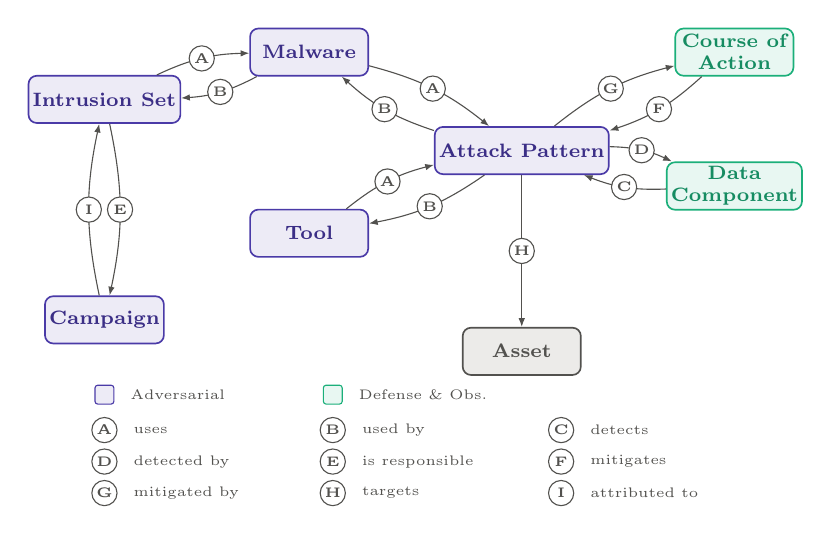
\begin{tikzpicture}[
  adv/.style={draw=titanAdversarial, rounded corners=3pt, align=center,
              minimum height=6mm, minimum width=15mm, inner sep=1.5pt,
              font=\scriptsize\bfseries, line width=0.6pt,
              fill=titanAdversarial!10, text=titanAdversarial!80!black},
  defbox/.style={draw=titanDefense, rounded corners=3pt, align=center,
              minimum height=6mm, minimum width=15mm, inner sep=1.5pt,
              font=\scriptsize\bfseries, line width=0.6pt,
              fill=titanDefense!10, text=titanDefense!80!black},
  tgt/.style={draw=titanNeutral, rounded corners=3pt, align=center,
              minimum height=6mm, minimum width=15mm, inner sep=1.5pt,
              font=\scriptsize\bfseries, line width=0.6pt,
              fill=titanNeutralLight!50, text=titanNeutral},
  fwd/.style={-{Latex[length=1.1mm]}, draw=titanNeutral, thin},
  badge/.style={circle, draw=titanNeutral, fill=white, minimum size=3.2mm,
                inner sep=0pt, font=\tiny\bfseries, text=titanNeutral},
  swatch/.style={rounded corners=1pt, minimum width=2.4mm, minimum height=2.4mm, inner sep=0pt},
  legtxt/.style={font=\tiny, text=titanNeutral, anchor=west},
]
% --- adversarial cluster ---
\node[adv] (is)   at (0,1.4)    {Intrusion Set};
\node[adv] (cam)  at (0,-1.4)   {Campaign};
\node[adv] (mal)  at (2.6,2.0)  {Malware};
\node[adv] (tool) at (2.6,-0.3) {Tool};
\node[adv] (ap)   at (5.3,0.75) {Attack Pattern};

% --- defense / observation cluster ---
\node[defbox] (coa) at (8.0,2.0)  {Course of\\Action};
\node[defbox] (dc)  at (8.0,0.3)  {Data\\Component};

% --- target ---
\node[tgt] (asset) at (5.3,-1.8) {Asset};

% --- typed, bidirectional edges: each pair is two single-headed arcs (one
% per direction), each carrying a letter badge for its relation (legend
% below). uses/used\_by cover several source types (Section~\ref{sec:benchmark:ontology});
% targets is the one relation with no inverse.
\draw[fwd, bend left=12] (is)   to node[badge, pos=0.5] {A} (mal);
\draw[fwd, bend left=12] (mal)  to node[badge, pos=0.5] {B} (is);

\draw[fwd, bend left=12] (cam)  to node[badge, pos=0.5] {I} (is);
\draw[fwd, bend left=12] (is)   to node[badge, pos=0.5] {E} (cam);

\draw[fwd, bend left=12] (mal)  to node[badge, pos=0.5] {A} (ap);
\draw[fwd, bend left=12] (ap)   to node[badge, pos=0.5] {B} (mal);

\draw[fwd, bend left=12] (tool) to node[badge, pos=0.5] {A} (ap);
\draw[fwd, bend left=12] (ap)   to node[badge, pos=0.5] {B} (tool);

\draw[fwd, bend left=12] (coa)  to node[badge, pos=0.5] {F} (ap);
\draw[fwd, bend left=12] (ap)   to node[badge, pos=0.5] {G} (coa);

\draw[fwd, bend left=12] (dc)   to node[badge, pos=0.5] {C} (ap);
\draw[fwd, bend left=12] (ap)   to node[badge, pos=0.5] {D} (dc);

\draw[fwd] (ap) to node[badge, pos=0.5] {H} (asset);

% --- legend: role swatches, then the letter code (3x3) ---
\node[swatch, fill=titanAdversarial!10, draw=titanAdversarial] (legadv) at (0,-2.35) {};
\node[legtxt, right=0.8mm of legadv] {Adversarial};
\node[swatch, fill=titanDefense!10, draw=titanDefense] (legdef) at (2.9,-2.35) {};
\node[legtxt, right=0.8mm of legdef] {Defense \& Obs.};

\node[badge] (lA) at (0,-2.8)   {A}; \node[legtxt, right=0.8mm of lA] {uses};
\node[badge] (lB) at (2.9,-2.8) {B}; \node[legtxt, right=0.8mm of lB] {used by};
\node[badge] (lC) at (5.8,-2.8) {C}; \node[legtxt, right=0.8mm of lC] {detects};
\node[badge] (lD) at (0,-3.2)   {D}; \node[legtxt, right=0.8mm of lD] {detected by};
\node[badge] (lE) at (2.9,-3.2) {E}; \node[legtxt, right=0.8mm of lE] {is responsible};
\node[badge] (lF) at (5.8,-3.2) {F}; \node[legtxt, right=0.8mm of lF] {mitigates};
\node[badge] (lG) at (0,-3.6)   {G}; \node[legtxt, right=0.8mm of lG] {mitigated by};
\node[badge] (lH) at (2.9,-3.6) {H}; \node[legtxt, right=0.8mm of lH] {targets};
\node[badge] (lI) at (5.8,-3.6) {I}; \node[legtxt, right=0.8mm of lI] {attributed to};
\end{tikzpicture}
\caption{TITAN Ontology, by role. Each labeled arc is one typed relation (legend below); \texttt{uses}/\texttt{used~by} letters cover several source types (e.g.\ malware, tool $\to$ attack pattern), spelled out in full in Appendix~\ref{sec:appendix}, which also lists Data Source and the remaining relation instances omitted here for space.}
\label{fig:ontology}
\end{figure*}

\subsection{Dataset Construction}
\label{sec:benchmark:dataset}

The benchmark is generated from 454 hand-written question templates, each carrying typed placeholders (e.g.\ \texttt{[malware]}) and a gold relational path over the ontology; because a path depends only on the node \emph{types} it touches, not on the specific entities filling them, one template yields many training instances as its placeholders are bound to different graph entities. Templates are paraphrased with an LLM (CITAZIONE) to add linguistic variety and discourage the planner from keying on surface template patterns rather than the underlying relation. Some questions have no single explicit starting node --- e.g.\ \emph{"List all ransomware detection strategies"}, where every ransomware instance is a valid start --- and for these the gold path uses one of the four operators (\texttt{filter}, \texttt{select}, \texttt{exec\_common}, \texttt{exec\_difference}) introduced in Section~\ref{sec:methodology:dsl}. Each instance also carries a chain-of-thought rationale that walks the path one relation at a time before stating the final program, used for the CoT reasoning-style condition (Section~\ref{sec:methodology:regimes}).

\subsection{Splits and Statistics}
\label{sec:benchmark:splits}

The benchmark is split into train (65{,}529 rows), validation (3{,}855), and test (15{,}627), for a total of 85{,}011 question--path pairs. The test split is template- and skeleton-disjoint from train and validation --- no test question shares its underlying template, nor a train row's relation skeleton, with anything the model is trained on --- which we verify independently by re-deriving each row's template and skeleton keys directly from its path text rather than trusting a stored split label. Table~\ref{tab:dataset_profile} breaks each split down by path length and by operator; the test split is, by construction, weighted toward longer paths and rarer operators than train (e.g.\ \texttt{select} and \texttt{exec\_difference} each make up roughly twice the share of test that they do of train), which makes it a meaningfully harder distribution, not merely a held-out sample of the same one.

\begin{table*}[t]
\centering
\small
\setlength{\tabcolsep}{4pt}
\begin{tabular}{lrrrr|rrrrr}
\toprule
& \multicolumn{4}{c}{\textit{Path length}} & \multicolumn{5}{c}{\textit{Operator}} \\
\cmidrule(lr){2-5}\cmidrule(lr){6-10}
\textbf{Split} & L1 & L2 & L3 & L4+ & filter & select & com. & diff. & plain \\
\midrule
Train & 27{,}048 & 26{,}247 & 6{,}535 & 5{,}699 & 18{,}634 & 951 & 1{,}336 & 176 & 44{,}432 \\
Val   & 1{,}619  & 1{,}490  & 411    & 335    & 1{,}091  & 56  & 80    & 9   & 2{,}619 \\
Test  & 5{,}984  & 5{,}425  & 1{,}732 & 2{,}486 & 4{,}599  & 485 & 44    & 150 & 10{,}349 \\
\bottomrule
\end{tabular}
\caption{Dataset profile by split (\texttt{com.}~=~\texttt{exec\_common}, \texttt{diff.}~=~\texttt{exec\_difference}, \texttt{plain}~=~no operator).}
\label{tab:dataset_profile}
\end{table*}


\section{Methodology}
\label{sec:methodology}

We ask whether the choice of \emph{target formalism} for LLM-generated graph queries interacts with the \emph{adaptation regime} under which the model is used. To isolate this interaction, we hold the reasoning task, the underlying knowledge graph, and the supervision fixed, and vary only two things: the surface language the planner is asked to produce, and whether the planner is prompted or fine-tuned.

\subsection{Problem Formulation}
\label{sec:methodology:formulation}

Given the TITAN knowledge graph $G=(V,E,R)$, typed, bidirectional relations $R$ over nodes $V$, described fully in Section~\ref{sec:benchmark}, and a natural-language question $q$, the task is to produce a program $P$ in a target formalism $F$ such that executing $P$ on $G$ returns an answer set $A \subseteq V$ satisfying $q$. We study two choices of $F$: a compact path DSL introduced by TITAN (Section~\ref{sec:methodology:dsl}), and SPARQL (CITAZIONE), obtained by a validated compilation of the same underlying supervision (Section~\ref{sec:methodology:sparql}). Because both formalisms execute equivalent supervision over equivalent graph representations, any performance gap we observe between $F{=}\text{DSL}$ and $F{=}\text{SPARQL}$ is attributable to the formalism itself and its interaction with the adaptation regime, not to unequal supervision (Figure~\ref{fig:pipeline}).

\begin{figure}[t]
\centering
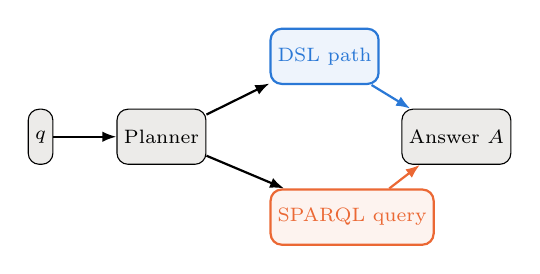
\begin{tikzpicture}[
  node distance=4mm and 8mm,
  box/.style={draw, rounded corners, align=center, minimum height=7mm,
              inner sep=2.5pt, font=\scriptsize},
  neutralbox/.style={box, fill=titanNeutralLight!50},
  dslbox/.style={box, draw=titanDSL, thick, text=titanDSL, fill=titanDSL!8},
  sparqlbox/.style={box, draw=titanSPARQL, thick, text=titanSPARQL, fill=titanSPARQL!8},
  arr/.style={-{Latex[length=1.8mm]}, thick},
]
\node[neutralbox] (q) {$q$};
\node[neutralbox, right=of q] (planner) {Planner};
\node[dslbox, above right=3mm and 8mm of planner] (dsl) {DSL path};
\node[sparqlbox, below right=3mm and 8mm of planner] (sparql) {SPARQL query};
\coordinate (mid) at ($(dsl)!0.5!(sparql)$);
\node[neutralbox, right=8mm of mid] (ans) {Answer $A$};

\draw[arr] (q) -- (planner);
\draw[arr] (planner) -- (dsl);
\draw[arr] (planner) -- (sparql);
\draw[arr, titanDSL] (dsl) -- (ans);
\draw[arr, titanSPARQL] (sparql) -- (ans);
\end{tikzpicture}
\caption{Same planner input and supervision; only the target formalism differs.}
\label{fig:pipeline}
\end{figure}

\subsection{The TITAN Path DSL}
\label{sec:methodology:dsl}

A DSL program is a step sequence, serialized as \texttt{<PATH>}~step$_1$~\texttt{<SEP>}~\ldots~\texttt{<SEP>}~step$_n$~\texttt{</PATH>}, and each step plays one of five roles. A \emph{relation} step (e.g.\ \texttt{uses\_attack\_pattern}) traverses a typed, bidirectional edge; a \emph{type seed} (\texttt{is\_<type>\_type}) restricts the current frontier to nodes of a given type, or initializes it if none exists yet; \texttt{filter~<keyword>} keeps only the nodes whose associated text satisfies a condition; \texttt{select~<entities>} forks execution into one parallel branch per named entity; and \texttt{exec\_common} / \texttt{exec\_difference} recombine the branches opened by the most recent \texttt{select}, by intersection or symmetric difference respectively. Execution is fully deterministic, which is what lets us score path correctness by direct execution rather than by comparing generated text to a single reference string (Section~\ref{sec:methodology:metrics}).

\subsection{Compiling to SPARQL}
\label{sec:methodology:sparql}

For the comparison to be fair, the SPARQL condition must express the same reasoning content as the DSL.

\paragraph{RDF projection.} $G$ is exported to an RDF graph (N-Triples) that carries over every typed relation edge together with the STIX literal properties (e.g.\ \texttt{name}, \texttt{description}) that SPARQL needs in order to filter and project results. The resulting projection comprises 128{,}026 triples over 27{,}568 distinct subjects and 69 distinct predicates.\footnote{Verified directly against the released \texttt{titan\_graph.nt}; the predicate set includes both the DSL's relation labels and STIX metadata literals the native executor never needs.}

\paragraph{Compilation.} A rule-based compiler maps every gold DSL path to a canonical SPARQL query, mirroring the DSL executor construct-by-construct: entity seeding becomes a bound-subject triple pattern, a relation step a predicate triple pattern, a type seed a type-restricting pattern, \texttt{filter} a \texttt{FILTER} clause, \texttt{select} a set of per-entity variable bindings, and \texttt{exec\_common}/\texttt{exec\_difference} a shared-variable join or a \texttt{MINUS}/\texttt{UNION} combination. These compiled queries supply the few-shot exemplars, the worked examples, and the fine-tuning targets for the SPARQL condition, so the DSL and SPARQL models are exposed to exactly the same underlying reasoning instances.

\paragraph{Validation.} We validate the compiler by executing, on a stratified sample of gold-executable rows, both the native DSL path and its compiled SPARQL counterpart, and comparing the two answer sets independently. The two executions agree on 100.00\% of two independent validation samples (1{,}500 and 4{,}000 rows). This is the basis for treating any DSL/SPARQL gap reported later as a property of the formalism, not an artifact of the comparison.

\subsection{Graph Execution}
\label{sec:methodology:executor}

DSL programs execute deterministically over $G$'s typed adjacency structure; SPARQL queries execute against the RDF projection through a compiled query engine.\footnote{We use \texttt{pyoxigraph} for the throughput it offers at our test-set scale.} Both paths converge on the same output type (a node/entity answer set) which is what every metric in Section~\ref{sec:methodology:metrics} ultimately scores.

\subsection{Prompted and Fine-Tuned Regimes}
\label{sec:methodology:regimes}

We cross three factors: \textbf{formalism} (DSL vs.\ SPARQL), \textbf{adaptation regime} (prompted vs.\ fine-tuned), and \textbf{reasoning style} (NoCoT vs.\ CoT; CITAZIONE), summarized in Table~\ref{tab:design}. The full $2{\times}2{\times}2$ grid is completed on a small set of backbones chosen specifically to isolate the formalism$\times$regime interaction.

\begin{table}[t]
\centering
\small
\begin{tabular}{ll}
\toprule
\textbf{Factor} & \textbf{Levels} \\
\midrule
Formalism & DSL, SPARQL \\
Regime & Prompted, Fine-tuned \\
Reasoning style & NoCoT, CoT \\
\bottomrule
\end{tabular}
\caption{Experimental design: three crossed factors.}
\label{tab:design}
\end{table}

\paragraph{Prompted.} The planner receives a schema description of the relation/predicate vocabulary and node types, derived programmatically from $G$ so that the DSL and SPARQL versions carry identical information content, together with 12 few-shot exemplars stratified by question category and 3 fixed worked examples. The NoCoT and CoT variants of a given prompt are identical except for a single closing instruction sentence, respond with only the program, or reason step by step first, which we ablate in isolation in Appendix~\ref{sec:appendix}.

\paragraph{Fine-tuned.} We fine-tune with LoRA (rank 16, $\alpha{=}16$, dropout 0), learning rate $3\times10^{-4}$ on a linear schedule, effective batch size 16, for up to 8 epochs with early stopping on validation loss.

\paragraph{Backbones.} We evaluate seven instruction-tuned LLMs spanning roughly two orders of magnitude in parameter count: Phi-3.5-mini (3.8B), Qwen2.5-7B, Qwen2.5-7B-Instruct, Qwen2.5-72B, Llama-3.3-70B, GPT-OSS-120B, and DeepSeek-R1-Distill-Llama-70B. Phi-3.5-mini and Qwen2.5-7B are fine-tuned under both formalisms and both reasoning styles; the remaining backbones are evaluated only in the prompted regime. Full per-model configuration is given in Appendix~\ref{sec:appendix}.

\subsection{Evaluation Metrics}
\label{sec:methodology:metrics}

\paragraph{Exact match (EM).} Path EM is the exact match between the predicted and reference DSL step sequences, after whitespace normalization; Query EM is the same comparison between the generated SPARQL text and the canonical query compiled from the reference path (Section~\ref{sec:methodology:sparql}).

\paragraph{Entity-level F1.} We execute the predicted program from the reference starting entities (oracle entity linking) and compare the resulting answer set to the one produced by the reference program, which isolates program quality from entity-resolution noise. F1 is undefined when the reference program itself yields an empty answer set, so we compute it, uniformly across every model and condition, only over gold-executable rows.


\section{Experimental Setup}
\label{sec:expsetup}
TODO --- models, decoding, compute budget (largely a restatement/tabulation of what Section~\ref{sec:methodology} already specifies, plus anything execution-specific).

\section{Results}
\label{sec:results}
TODO --- main results table; the 2$\times$2 reversal schematic; length/operator heatmap; CoT fine-tuning reversal (diverging bars); paraphrase-robustness dumbbell chart.

\section{Discussion}
\label{sec:discussion}
TODO --- mechanism discussion for why prompting favors the DSL and fine-tuning favors SPARQL; the CoT-fine-tuning asymmetry; EM/F1 dissociation.

\section{Limitations}
\label{sec:limitations}
TODO --- RAG baseline and human/analyst plausibility evaluation are explicitly scoped out here as future work (code/infrastructure exists but was not run for this paper), not silently omitted. Also: single domain (CTI), synthetic template origin, paraphrase degradation.

\section{Conclusion}
\label{sec:conclusion}
TODO.

% No \cite commands are used in this draft; every citation point is marked
% with the literal placeholder CITAZIONE per drafting instructions.
% \bibliography{bibliography}
% \bibliographystyle{acl_natbib}

\appendix
\section{Additional Experimental Details}
\label{sec:appendix}
TODO --- per-model decoding/quantization/compute configuration; instruction-wording ablation table (Section~\ref{sec:methodology:regimes}); full length$\times$operator numeric tables; per-section dataset breakdown; full ontology node/edge/relation counts (Table~\ref{tab:ontology_counts}, referenced from Section~\ref{sec:benchmark:ontology}).

\end{document}
